\section{Dynamik}
\subsection{Geradlinig(Translation)}
\begin{boxshaded}
\begin{align*}
&\text{1.Trägheitgesetz}\quad \sum{vm}=\text{const}& &\text{Geschlossenes System} \\
&\text{2.Grundgesetz Mechanik}\quad \sum{F}=ma& &\text{Summen aller Kräfte gleich Trägheit} \\
&\text{3.Wechselwirkunggesetz}\quad \vv{F}_{21}=-\vv{F}_{12}& &\text{Aktion gleich Reaktion} 
\end{align*}
\end{boxshaded}

\begin{boxleft}\bla{Kraft}
\des[\newton]{F}{Kraft}\\
\des[\kilo\gram]{m}{Masse}
\end{boxleft}\begin{boxrightshaded}
\begin{align*}
\vv{F}&=m\cdot \vv{a}\\
\vv{F}_{\text{Tr}}&=-m\cdot \vv{a}\\
\vv{F}&=\frac{\diff p}{\diff t}\vv{e}_p=\frac{\diff}{\diff t}\left(mv\right)\vv{e}_v
\end{align*}
\end{boxrightshaded}

\begin{boxleft}\bla{Impuls}
\des[\kilo\gram\meter\per\second]{p}{Impuls}
\end{boxleft}\begin{boxrightshaded}
\begin{align*}
\vv{p}&=m\cdot \vv{v}
\end{align*}
\end{boxrightshaded}

\begin{boxleft}\bla{Kraftstoß}
\end{boxleft}\begin{boxrightshaded}
\begin{align*}
\vv{F}&=\frac{\diff \vv{p}}{\diff t}=m\cdot\frac{\diff \vv{v}}{\diff t}+\vv{v}\cdot\frac{\diff m}{\diff t}\\
\Delta\vv{p}&=\vv{p}_2-\vv{p}_1=\int_{\vv{p}_2}^{\vv{p}_1}\diff p=\int_0^{t}\vv{F}\diff t
\end{align*}
\end{boxrightshaded}

\begin{boxleft}\bla{Arbeit}
\des[\kilo\gram\meter\tothe{2}\per\second\tothe{2}]{W}{Arbeit}
\end{boxleft}\begin{boxrightshaded}
\begin{align*}
W&=-\int_{\vv{s}_1}^{\vv{s}_2}\vv{F_{\text{Tr}}}\circ\diff \vv{s}\\
&=\int_{\vv{v}_0}^{\vv{v}_1}m\vv{v}\circ\diff \vv{v}=\frac{1}{2}m\left(v_1^2-v_0^2\right) 
\end{align*}
\end{boxrightshaded}

\begin{boxleft}\bla{kin. Energie}
\des[\kilo\gram\meter\tothe{2}\per\second\tothe{2}]{E}{Energie}
\end{boxleft}\begin{boxrightshaded}
\begin{align*}
E_{\text{kin}}=\frac{1}{2}mv^2
\end{align*}
\end{boxrightshaded}


\begin{boxleft}\bla{Hubarbeit}
\des[\meter\per\second\tothe{2}]{g}{Fallbeschleunigung}
\end{boxleft}\begin{boxrightshaded}
\begin{align*}
W_{\text{hub}}&=mgh
\end{align*}
\end{boxrightshaded}

\begin{boxleft}\bla{Leistung}
\des[\kilo\gram\meter\tothe{2}\per\second\tothe{3}]{g}{Leistung}
\end{boxleft}\begin{boxrightshaded}
\begin{align*}
P=\vv{F}\circ\vv{v}=\frac{\diff W}{\diff t}=\dot{W}
\end{align*}
\end{boxrightshaded}


\subsection{Drehbewegung(Rotation)}

\begin{boxleft}\bla{Massenträgheitsmoment}
\des[\kilo\gram\meter\tothe{2}]{J}{Massenträgheitsmoment}
\end{boxleft}\begin{boxrightshaded}
\begin{align*}
J=\int r^2 \diff m
\end{align*}
\end{boxrightshaded}

\begin{boxleft}\bla{Drehimpuls}
\des[\kilo\gram\meter\tothe{2}\radian\per\second]{L}{Drehimpuls}
\end{boxleft}\begin{boxrightshaded}
\begin{align*}
\vv{L}&=\vv{r}\times\vv{p} \\
&=J\cdot \vv{\omega}
\end{align*}
\end{boxrightshaded}

\begin{boxleft}\bla{Drehmoment}
\des[\newton\meter]{M}{Drehmoment}
\end{boxleft}\begin{boxrightshaded}
\begin{align*}
\vv{M}&=\vv{r}\times\vv{F}=J\vv{\alpha}=\dot{\vv{L}}
\end{align*}
\end{boxrightshaded}

\begin{boxleft}\bla{kinetische Energie}
\end{boxleft}\begin{boxrightshaded}
\begin{align*}
E_{kin}=\frac{1}{2}J\omega^2
\end{align*}
\end{boxrightshaded}

\begin{boxleft}\bla{Arbeit}
\end{boxleft}\begin{boxrightshaded}
\begin{align*}
W	&=\int_{\varphi_0}^{\varphi_1}\vv{M}\circ\vv{e_\omega}\diff \varphi=\int_{\vv{\omega}_0}^{\vv{\omega}_1}J\vv{\omega}\diff\vv{\omega}\\
&=\frac{1}{2}J\left(\omega_1^2-\omega_0^2\right)
\end{align*}
\end{boxrightshaded}


\begin{boxleft}\bla{Leistung}
\end{boxleft}\begin{boxrightshaded}
\begin{align*}
P=\vv{M}\circ\vv{\omega}
\end{align*}
\end{boxrightshaded}

\begin{boxleft}\bla{Zentripedalkraft}
\end{boxleft}\begin{boxrightshaded}
\begin{align*}
\vv{F}_{zp}&=-m\cdot\omega^2\cdot r\vv{e_r}\\
&=-m\cdot v^2\cdot \frac{\vv{e}_r}{r}
\end{align*}
\end{boxrightshaded}

\subsection{Schiefe Ebene}

\begin{boxleft}\bla{Kräfte}
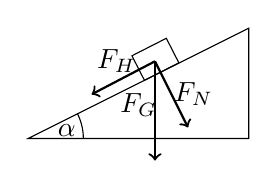
\begin{tikzpicture}[scale=.7]
  \draw (0,0) -- (4,0) -- (4,2)-- cycle;
  \draw[yshift=30,xshift=60,rotate=27] (0,0) -- (0,.5) -- (.7,.5) -- (.7,0) --cycle;
    
  \draw (1,0) arc (0:27:1);
  \draw (.7,0.15)node{$\alpha$};

  \draw[thick,->] (2.3,1.4)--(2.3,-.4);
  \draw[thick,->] (2.3,1.4)--(1.15,.8);
  \draw[thick,->] (2.3,1.4)--(2.9,.2);

  \draw (1.6,1.4)node{$\vv{F}_H$};
  \draw (3,0.8)node{$\vv{F}_N$};
  \draw (2,0.6)node{$\vv{F}_G$};
\end{tikzpicture}
\end{boxleft}\begin{boxrightshaded}
\begin{align*}
\vv{F}_N&=\vv{F}_G\cos\alpha\\
\vv{F}_H&=\vv{F}_G\sin\alpha
\end{align*}
\end{boxrightshaded}

\subsection{Reibung}

\begin{boxleft}\bla{Reibungskräfte}
\des[\newton]{F_N}{Normalkraft}\\
\des[\newton]{F_R}{Reibungskraft}\\
\des{\mu}{Reibungskoeffizient}
\end{boxleft}\begin{boxrightshaded}
\begin{align*}
F_R=\mu\cdot F_N
\end{align*}
\end{boxrightshaded}

\begin{boxleft}\bla{Rollreibung}
\des[\newton]{F_N}{Normalkraft}\\
\des{f}{Rollreibungstahl}\\
\des{M}{Drehmoment}\\
\des[\meter]{r}{Radius}
\end{boxleft}\begin{boxrightshaded}
\begin{align*}
M&=f\cdot F_N\\
F_R&=\frac{f}{r}\cdot F_N
\end{align*}
\end{boxrightshaded}

\subsection{Feder}

\begin{boxleft}\bla{Hookesches Gesetz}
\des[\newton\per\meter]{k}{Federkonstante}\\
\des[\newton\meter\per\radian]{D}{Winkelrichtgröße}
\end{boxleft}\begin{boxrightshaded}
\begin{align*}
F&=-kx\\
M&=-D\varphi
\end{align*}
\end{boxrightshaded}

\begin{boxleft}\bla{Spannungsenergie}
\end{boxleft}\begin{boxrightshaded}
\begin{align*}
W	&=\int_{x_\text{min}}^{x_\text{max}}F\diff x=\int_{x_\text{min}}^{x_\text{max}}kx\diff x\\
	&=\frac{1}{2}\cdot k\cdot \left(x_{\text{max}}^2-x_{\text{min}}^2\right)
\end{align*}
\end{boxrightshaded}

\subsection{Elastischer Stoß}

\begin{boxleft}\bla{Energieerhaltung}
\end{boxleft}\begin{boxrightshaded}
\begin{align*}
\text{Energie vor den Stoß} &= \text{Energie nach den Stoß}\nonumber\\
\sum E_{\text{kin}}&=\sum E_{\text{kin}}'
\end{align*}
\end{boxrightshaded}

\begin{boxleft}\bla{Impulserhaltung}
\end{boxleft}\begin{boxrightshaded}
\begin{align*}
\text{Impuls vor den Stoß} &= \text{Impuls nach den Stoß}\nonumber\\
\sum m\vv{v}&= \sum m\vv{v}'
\end{align*}
\end{boxrightshaded}

\begin{boxleft}\bla{Zentraler, elastischer Stoß}
\destext{(Energie und Impuls)}
\end{boxleft}\begin{boxrightshaded}
\begin{align*}
\frac{1}{2}m_1v_1^2+\frac{1}{2}m_2v_2^2&=\frac{1}{2}m_1v_1'^2+\frac{1}{2}m_2v_2'^2\\
m_1v_1+m_2v_2&=m_1v_1'+m_2v_2'
\end{align*}
\end{boxrightshaded}

\begin{boxleft}\bla{Zentraler, elastischer Stoß}
\destext{(Geschwindigkeit nach dem Stoß)}
\end{boxleft}\begin{boxrightshaded}
\begin{align*}
v_2'&=\frac{2m_1}{m_1+m_2}v_1+\frac{m_2-m_1}{m_1+m_2}v_2\\
v_1'&=\frac{2m_2}{m_1+m_2}v_2+\frac{m_1-m_2}{m_1+m_2}v_1
\end{align*}
\end{boxrightshaded}

\subsection{Unelastischer Stoß}

\begin{boxleft}\bla{Energieerhaltung}
\end{boxleft}\begin{boxrightshaded}
\begin{align*}
\text{Energie vor den Stoß} &= \text{Energie nach den Stoß}+\text{Arbeit}\nonumber\\
\sum E_{\text{kin}}&=\sum E_{\text{kin}}'+\Delta W
\end{align*}
\end{boxrightshaded}

\begin{boxleft}\bla{Impulserhaltung}
\end{boxleft}\begin{boxrightshaded}
\begin{align*}
\text{Impuls vor den Stoß} &= \text{Impuls nach den Stoß}\nonumber\\
\sum m\vv{v}&= \sum m\vv{v}'
\end{align*}
\end{boxrightshaded}

\begin{boxleft}\bla{Total unelastischer Stoß}
\destext{(Energie und Impuls)}
\end{boxleft}\begin{boxrightshaded}
\begin{align*}
\frac{1}{2}m_1v_1^2+\frac{1}{2}m_2v_2^2&=\frac{1}{2}\left(m_1+m_2\right)v'^2+\Delta W\\
m_1v_1+m_2v_2&=\left(m_1+m_2\right)v'
\end{align*}
\end{boxrightshaded}

\begin{boxleft}\bla{Total unelastischer Stoß}
\destext{(Geschwindigkeit nach dem Stoß)}
\end{boxleft}\begin{boxrightshaded}
\begin{align*}
v'		&=\frac{m_1v_1+m_2v2}{m_1+m_2}
\end{align*}
\end{boxrightshaded}

\begin{boxleft}\bla{Total unelastischer Stoß}
\destext{(Energieverlust)}
\end{boxleft}\begin{boxrightshaded}
\begin{align*}
\Delta W	&=\frac{m_1\cdot m_2}{2\left(m_1+m_2\right)}\left(v_1-v_2\right)^2
\end{align*}
\end{boxrightshaded}
\subsection{Drehimpulse}

\begin{boxleft}\bla{Drehimpulserhaltungssatz}
\end{boxleft}\begin{boxrightshaded}
\begin{align*}
\text{Drehinpuls zur Zeit 1} &= \text{Drehimpuls zur Zeit 2}\\
\sum \vv{L}&=\sum \vv{L}'
\end{align*}
\end{boxrightshaded}

\begin{boxleft}\bla{Kupplung Zweier Drehkörper}
\destext{(Winkelgeschwindigkeit nach dem Kuppeln und Energieverlust)}
\end{boxleft}\begin{boxrightshaded}
\begin{align*}
\vv{\omega}'&=\frac{J_0\vv{\omega_0}+J_1\vv{\omega_1}}{J_1+J_2}\\
W&=\frac{J_0\cdot J_1}{2\left(J_0+J_1\right)}\left(\omega_0-\omega_1\right)^2
\end{align*}
\end{boxrightshaded}


\subsection{Rotierendes Bezugssystem}

\begin{boxleft}\bla{Zentrifugalkraft}
\end{boxleft}\begin{boxrightshaded}
\begin{align*}
\vv{F}_Z&=F_r\cdot \vv{e}_r=-m\vv{\omega}\times\left(\vv{\omega}\times\vv{r}\right)=-m\vv{\omega}\times\vv{v}\\
  F_Z&=-m\frac{v^2}{r}=-m\omega^2 r
\end{align*}
\end{boxrightshaded}

\begin{boxleft}\bla{Corioliskraft}
\end{boxleft}\begin{boxrightshaded}
\begin{align*}
\vv{F}_C&=-2m\vv{\omega}\times\vv{v}
\end{align*}
\end{boxrightshaded}
